\subsection{Overview}
Some lectures overview:
\begin{outline}
    \1 Algorithm fundamentals of search
        \2 Intro AI and Rational agents
        \2 Uniformed Search
        \2 Informed Search
    \1 Applications of search in deterministic environments
        \2 CSP
        \2 Pattern Mining
        \2 Game Tree
        \2 Planning
    \1 Application of search in stochastic environments
        \2 Markov Decision Processes
    \1 BDA
        \2 Intro to logic
        \2 SAT solving
        \2 Local Search
\end{outline}

\noindent
The planning we learn is \textbf{Goal Oriented Action Planning: STRIPS Planning.} Search for a plan that achieves that goal in the current state.

\subsection{STRIPS planning}
\subsubsection{Overview}
Typical description of a planning problem:
\begin{outline}
    \1 Initial state
    \1 Goal
    \1 Available actions
\end{outline}

\noindent
Typical solution of a planning problem: a sequence of actions when excuted in the initial state results in a state that satisfies the goal condition. (\textbf{A sequence of actions} that achieves the goal for \textbf{every application domain})

\noindent
Planning: the automatic discovery of such solutions. (\textbf{Find} such sequence of actions that achieves the goal for every application domain)

\subsubsection{Example: Blocks world domain}
\begin{outline}
    \1 Initial state: $s_{0}$
    \1 Goal: $g$
    \1 Available actions:
        \2 $move(A,table,B)$: move A from table to top of B
        \2 $move(A,B,table)$: move A from top of B to table
        \2 $move(A,C,B)$: move A from top of C to top of B (not from table)
\end{outline}

\begin{figure}[htbp]
    \centering
    \begin{subfigure}[t]{0.25\textwidth}
        \centering
        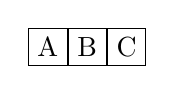
\begin{tikzpicture}
            \node [draw,rectangle](a)at(-1/2,0){A};
            \node [draw,rectangle](b)at(0,0){B};
            \node [draw,rectangle](c)at(1/2,0){C};     
        \end{tikzpicture}
        \caption{Initial state $s_{0}$}
        \label{fig:initial_state_in_BWD}
    \end{subfigure}
    \begin{subfigure}[t]{0.25\textwidth}
        \centering
        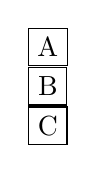
\begin{tikzpicture}
            \node [draw,rectangle](a)at(0,1){A};
            \node [draw,rectangle](b)at(0,1/2){B};
            \node [draw,rectangle](c)at(0,0){C};     
        \end{tikzpicture}
        \caption{Goal state $g$}
        \label{fig:goal_state_in_BWD}
    \end{subfigure}
    \caption{Initial state and Goal state for Blocks world domain}
    \label{fig:states_in_BWD}
\end{figure}

\noindent
In the beginning, we need to find a representation for the state and actions. For the state in blocks world is shown as below. For each state, the state should be \textbf{completely} specified based on the \textcolor{blue}{\textbf{Closed-World Assumption: any literal not mentioned in the description of the state are assumed to be false!}}.
\begin{outline}
    \1 On(b,x):
        \2 block b is on top of x, where x is another block 
    \1 Clear(x):
        \2 a block can be placed on the top of x
\end{outline}

\noindent
Thus, the initial state in Figure~\ref{fig:initial_state_in_BWD} are: $on(a,table)$, $on(b,table)$, $on(c,table)$, $clear(a)$, $clear(b)$, $clear(c)$. \textcolor{blue}{(Closed-World Assumption)} Additionally, the goal state in Figure~\ref{fig:goal_state_in_BWD} are: $clear(a)$, $on(a,b)$, $on(b,c)$, $on(c,table)$. \textcolor{blue}{(No Closed-World Assumption)}, we only need to satify the goal. (A state $s$ satisfies goal $g$ if it contains all literals in $g$, containing is okay, not exactly identified.)

\noindent
Next is the availble actions. It consists of \textbf{preconditions} and \textbf{effects}.
\begin{outline}
    \1 Preconditions: literals denoting what needs to be in the state for the action to be availble
    \1 Effects: literals denoting how the state is changing when action is applied
\end{outline}

\noindent
One of the avialble action is $move(b,x,y)$, meaning that move b from top of x to top of y. Anonther action can be $moveToTable(b,x)$ and $moveFromTable(b,x)$
\tabto{0mm} $move(b,x,y)$
\tabto{5mm} Preconditions:
\tabto{10mm} $on(b,x)$, $clear(b)$, $clear(y)$
\tabto{5mm} Effects:
\tabto{10mm} $\neg on(b,x)$, $\neg clear(y)$, $on(b,y)$, $clear(x)$ 
\tabto{0mm} $moveToTable(b,x)$
\tabto{5mm} Preconditions:
\tabto{10mm} $clear(b)$, $on(b,x)$
\tabto{5mm} Effects:
\tabto{10mm} $\neg on(b,x)$, $on(b,table)$, $clear(x)$
\tabto{0mm} $moveFromTable(b,x)$
\tabto{5mm} Preconditions:
\tabto{10mm} $clear(b)$, $clear(x)$
\tabto{5mm} Effects:
\tabto{10mm} $\neg on(b,table)$, $\neg clear(x)$, $on(b,x)$

\noindent
Why do we like formalism? Because it is easy for representation. STRIPS planning: finding a solution to the planning problem following a \textbf{state-based search:}
\begin{outline}
    \1 Init(\textcolor{orange}{where to start from})
    \1 Goal(\textcolor{orange}{when to stop searching})
    \1 Action(\textcolor{blue}{how to generate the "graph"})
\end{outline}

\noindent
When planning, there are two planning: 
\begin{outline}
    \1 Progression planning: forward state-based search \textcolor{red}{$\leftarrow$ mainly focus on}
    \1 Regression planning: backward state-based search
\end{outline}

\noindent 
The \textbf{\textcolor{blue}{pseudocode}} for progressing planning: - similar to backtracking
\begin{enumerate}
    \item Start from the initial state
    \item Check if the current state satisfies the goal
    \item Compute availble actions to the current state
    \item Compute the successor states
    \item Pick one of the \textbf{(not-visited)} successor states as the current state
    \item Repeat until a solution is found or the state space is exhausted \textcolor{red}{$\leftarrow$ similar to backtracking}
\end{enumerate}

\noindent
Is it guaranteed that progressive planning will find a solution if one exists? \textcolor{red}{$\leftarrow$ yes, if the state-space is finite} 

\noindent
But it will be very very slow, if we search the whole space-state (the worst case). \textcolor{red}{$\leftarrow$ heuristics needed!} We need heuristics that help progression planning pick the most promising states to investigate first

\subsection{Heuristics for STRIPS planning}
Analogy: $A^{*}$ search, evalution function = $f(s) = g(s) + h(s)$, where $g(s)$ from UCS and $h(s)$ from greedy search. Similar to the $A^{*}$ search, here we use $f(s)$ for STRIPS planning to pick the most promising one. Some of possible $h(s)$ and $g(s)$ can be as below. \emph{(Similarly, we need to check whether it is admissble heuristics to obtain the optimal solution)}
\begin{outline}
    \1 $g(s)$: number of literals that exists in the goal
    \1 $h(s)$: number of literals in the goal that are missing from s
\end{outline}

\noindent
The \textcolor{blue}{\textbf{pseudocode}} for \textcolor{blue}{\textbf{progressing planning}} applied with heuristics can be updated as below:
\begin{enumerate}
    \item Start from the initial state
    \item Check if the current state satisfies the goal
    \item Compute availble actions to the current state
    \item Compute the successor states
    \item Pick \textcolor{red}{\textbf{(the most promising}} successor states as the current state
    \item Repeat until a solution is found or the state space is exhausted \textcolor{red}{$\leftarrow$ similar to backtracking}
\end{enumerate}

\noindent
Alternatives: \textcolor{blue}{\textbf{pseudocode}} for \textcolor{blue}{\textbf{Regression planning }} is similar but invert the progressing planning:
\begin{enumerate}
    \item Start from the \textbf{goal} state as current state
    \item Check if the \textbf{initial state} satisfies the current state
    \item Compute the \textbf{relevant} and \textbf{consistent} actions for current state
    \item Compute the \textbf{predecessor} states (which is actually next state in this case)
    \item Pick \textcolor{red}{\textbf{(the most promising}} successor states as the current state
    \item Repeat until a solution is found from \textbf{goal state} to \textbf{initial state} or the state space is exhausted (no solution)
\end{enumerate}

\subsection{Summary}
\begin{enumerate}
    \item A generic formalism (easy to represent difficult space search, similar to ILP) for \textbf{representing} planning problem (a specific aspect in searching problem)
    \item Generic \textbf{search} procedures for finding a plan
    \begin{enumerate}
        \item Progressing planning (forward)
        \item Regression planning (backward, not discussed, only pseudocode)
    \end{enumerate}
    \item Application in many aspects, e.g., space, flight, robotics, etc.
\end{enumerate}


\pagebreak